\JWlone{Correctness and Security of the Protocol}
\label{sec:security}

This chapter states and proves the security of the protocol in the
\JWdef{Universal--Composability}{UC} framework by Ran Canetti \cite{canetti05}.
In the UC framework, security is defined by comparing an \emph{ideal model} to a
\emph{real model}. The ideal model implements the intended functionality
\JWfuncSym{}{} safely by definition. The protocol under examination runs in the
real model. In the real model, there is an adversary $\mathcal{A}$ that controls
all corrupted parties.  In the ideal model, there is a simulator $\mathcal{S}$
that tries to mimic $\mathcal{A}$. An environment $\mathcal{Z}$ is plugged to
either the real or the ideal model and has to guess to which it is plugged to. A
protocol \JWprotoSym{}{} is an universally composable implementation of the
ideal functionality if, for every adversary $\mathcal{A}$ there is a
simulator $\mathcal{S}$ such that for all environments $\mathcal{Z}$ the entire
view of $\mathcal{Z}$ in the real model (with \JWprotoSym{}{} and $\mathcal{A}$)
is statistically close to its view in the ideal model (with \JWfuncSym{}{} and
$\mathcal{S}$).

\begin{align*}
%
\forall \mathcal{A}\ \exists \mathcal{S}\ \forall \mathcal{Z} :
\text{ideal}\ \widetilde{=}\ \text{real}
%
\end{align*}

%
% PROTOCOL AND FUNCTIONALITY
%
%
% PROTOCOL DESCRIPTION
%
\JWlone{Protocol Description}
\label{sec:protocol}

\begin{JWfunc}%
  {\JWfuncSymOPE}%
  {The ideal $\JWfieldGeneral{}$-OPE functionality \JWfuncSymOPE{}}%
  {fig:func-ope}

  Parametrized by a finite field size $2^k$ and maximal polynomial degree $n$.

  \begin{JWfuncSteps}

  \item Upon receiving input \JWmsgTP{Commit}{$a$} from the environment, verify
    $a \in \JWfieldGeneral^n$ and that there is no stored input, yet; else
    ignore that input. Next record $a$.

  \item Upon receiving input \JWmsgTP{Evaluate}{$x$} from the enviconment,
    verify $x \in \JWfieldGeneral{}$ and that there is no stored input, yet;
    else ignore that input. Next record $x$.

  \item Upon $a$ and $x$ are verified and stored, compute $y \leftarrow
    \sum_{i=0}^n a_ix^i$ and output \JWmsgTP{Evaluated}{$y$}.

  \end{JWfuncSteps}
\end{JWfunc}

\begin{figure}[ht]

  \label{fig:graph-ope}
  \centering

  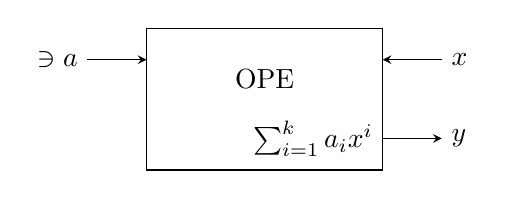
\begin{tikzpicture}[>=stealth]

    \node (OPE) at (8.5,0) {OPE};
    \draw (OPE) +(-1.5,-1.15) rectangle +(1.5,0.65);

    \draw [<-] (OPE) ++(-1.5,0.25) node [anchor=west] {} -- +(-0.75,0) node
    [anchor=east] {$\JWfieldGeneral \ni a$};

    \draw [<-] (OPE) ++(1.5,0.25) node [anchor=east] {} -- +(0.75,0) node
    [anchor=west] {$x$};

    \draw [->] (OPE) ++(1.5,-0.75) node [anchor=east] {$\sum_{i=1}^k a_ix^i$}
    -- +(0.75,0)
    node [anchor=west] {$y$};

  \end{tikzpicture}

  \caption{Graphical Representation of \JWfuncSymOPE}

\end{figure}

\begin{JWprotocol}%
  {\JWprotoSymOPE}%
  {Protocol: Oblivious Polynomial Evaluation}%
  {fig:proto-ope}

  Parametrized by the security parameter $k$ that specifies the field
  $\mathbb{F}_{2^k}$ and the maximal degree of the polynomial $n$.

  \JWprotoPhase{Setup:}

  \begin{JWprotoSteps}

  \item Upon input \JWmsgTP{Commit}{$a$} from the environment, \JWpOne{}
    verifies that $a \in \mathbb{F}_{2^k}^{n+1}$; else ignore that input. Next,
    \JWpOne{} generates the DRAC and sets up the OAFE functionality for the
    polynomial $f(x) = \sum_{i=0}^n a_ix^i$ (see section \ref{sec:OPE}).

  \item Finally, \JWpOne{} sends DRAC to \JWpTwo{}.

  \end{JWprotoSteps}


  \JWprotoPhase{Evaluation:}

  \begin{JWprotoSteps}

  \item Upon receiving the DRAC from \JWpOne{}, verify that there is no stored
    DRAC yet, else ignore that input. Next, \JWpTwo{} verifies the received
    input really it a DRAC, else ignore that input. Additionally it verifies
    that the DRAC encodes a function whose degree is less or equal than $n$ (see
    chapter \ref{sec:max-poly-degree}), else ignore the input. If the DRAC
    verification was successful, store the DRAC.

  \item Upon receiving input \JWmsgTP{Evaluate}{$x$} from the environment,
    verify that $x \in \mathbb{F}_{2^k}$, else ignore that input. If there is
    already a stored DRAC, continue at the next step, else wait for a stored
    DRAC.

  \item Next, \JWpTwo{} evaluates the DRAC. Because the OAFE functionality is
    set up by \JWpOne{}, during the evaluation it is possible that the OAFE
    functionality turns out to behave unexpectedly: It could decline needed
    evaluations and it could return vectors of unexpected shapes. In both cases
    always assume it would have returned all zero vectors of the expected shape.

  \item After the Evaluation, \JWpTwo{} adds both components of the last DRAV
    and queries a special final OAFE with that value. Again, assume the all zero
    vector is the OAFE behaves unexpectedly. The then received new value is the
    result of the computation $y = \sum_{i=1}^k a_ix^i$. Finally, output
    \JWmsgTP{Evaluated}{$y$} to the environment.

  \end{JWprotoSteps}

\end{JWprotocol}

% vim: set spell spelllang=en_us fileencoding=utf8 :


%
% SIMULATORS
%
\JWltwo{Simulators}
\label{sec:simulators}

This section describes two simulators which mimic some adversary \JWadv{} in the
ideal model. There is a separate simulator for each of the potentially corrupted
parties. The security proofs in Section \ref{sec:proof} will use these
simulators to proof the indistinguishability between the real model and the
ideal model.

% SIMULATOR S_DAVID(A)
\JWlthree{Simulator $\mathcal{S}_{\text{\JWpTwo{}}}(\mathcal{A})$}
\label{sec:simulator-david}

\paragraph{Setup Phase:}

\begin{itemize}

  \item Setup an emulated version of the given real model adversary
    \JWadv{} which especially impersonates the corrupted \JWpTwo{}.

  \item Setup emulated, honest \JWpOne{} labeled $\mathcal{G}$.

  \item Setup emulated, honest OAFE functionality labeled \JWfuncSymOAFE{}.

  \item Initialize $\mathcal{G}$ with a random polynomial of the parametrized
    degree $k$ and record the DRAC $C$ it generated.

  \item Wire $\mathcal{G}$, \JWfuncSymOAFE{} and \JWadv{} to each other
    and \JWadv{} to the environment as in the real model.

  \item Start the simulation by transitioning to the \emph{Processing Phase}.

\end{itemize}

\paragraph{Processing Phase:}

\begin{itemize}

  \item Intercept the adversary's (\JWadv{}) polynomial input $x$. This is
    trivial because it is the first message that \JWadv{} transmits to
    \JWfuncSymOAFE{} (only considering messages accepted by \JWfuncSymOAFE{}).
    Notice, this is the initial DRAV encoding of the plain value $x$. Next, halt
    the simulation and evaluate the proper polynomial using the intercepted
    input $x$ and the ideal functionality \JWfuncSymOPEnp{} by sending it
    \JWmsgTP{Evaluate}{$x$}.

  \item Upon receiving \JWmsgTP{Evaluated}{$y$} from \JWfuncSymOPEnp{},
    calculate the value $\chi$ with which an honest \JWpTwo{} would evaluate the
    last OAFE . Because an honest \JWpTwo{} acts entirely deterministic, this
    calculates from the stored DRAC $C$, the OAFE parameters in \JWfuncSymOAFE,
    and the stored input $x$. Next, draw a random value $r$ and calculate $\psi
    = \frac{y-r}{\chi}$. Next, reconfigure the parameters of the last OAFE to
    $(\psi, r)$. The last OAFE then calculates the affine function $f(\eta) =
    \psi \cdot \eta + r$ which---when evaluated with $\chi$---calculates the
    result $y$ of the proper polynomial at the node $x$. Since any honest
    \JWpTwo{} evaluates the last OAFE with $\chi$, it will receive the correct
    result $y = f(\chi) = \psi \cdot \chi + r = \frac{y-r}{\chi} \cdot \chi + r
    = y$. Any dishonest \JWpTwo{} will receive some random value depending on
    the random value $r$. Finally unhalt the simulation, no further
    interceptions are necessary.

\end{itemize}


% SIMULATOR S_Goliath(A)
\JWlthree{Simulator $\mathcal{S}_{\text{Goliath}}(\mathcal{A})$}
\label{sec:simulator-goliath}

The setup phase is run as soon as the simulator starts.

\paragraph{Setup Phase:}

\begin{itemize}

  \item Setup emulated, honest \JWpTwo{} and OAFE functionality
    \JWfuncSymOAFE{}.

  \item Wire the given real model adversary \JWadv{} that impersonates \JWpOne{}
    with the emulated \JWpTwo{} and \JWfuncSymOAFE{}. Additionally wire \JWadv{}
    with the environment the way they would be wired in the real model.

\end{itemize}

\paragraph{Processing Phase:}

\begin{itemize}

  \item Upon the emulated OAFE functionality received the OAFE configuration and
    the emulated \JWpTwo{} received the DRAC, symbolically evaluate the
    polynomial that \JWadv{} described. During the symbolic evaluation, the OAFE
    functionality configuration could proof to be unfitting: \JWadv{} could
    have sent a configuration that allows too few OAFE evaluations or evaluates
    to vectors of wrong shape. In both cases, modify the configuration to return
    all zero vectors of the correct shape whenever the DRAC evaluation would
    fail otherwise.

  \item After having symbolically evaluated the polynomial encoded by \JWadv{},
    verify, that the polynomial has a degree that equals the parametrized degree
    $k$. If \JWadv{} submitted a polynomial of valid degree, store the
    polynomial's coefficients as $a \in \JWfieldGeneral^n$.  Next, upload that
    polynomial to the ideal functionality \JWfuncSymOPEnp{} by sending
    \JWmsgTP{Commit}{$a$} to \JWfuncSymOPEnp{}, the simulation is now
    terminated, wait for the adversary to terminate as well. If the polynomial
    was illegal, restart the simulator in the setup phase.  This restart is
    equivalent to ignoring the adversary's inputs.

\end{itemize}


%
% PROOF
%
\JWltwo{Security Proof}
\label{sec:proof}

The proof is a distinction between the two relevant settings: Either \JWpOne{}
or \JWpTwo{} is corrupted. The proof below handles theses cases separately. The
remaining possibilities that either no party is corrupted or both parties are
corrupted do not have to be proved separately. No meaningful proof is possible
if both parties are corrupted and no proof is necessary if all involved parties
act honest.


% CORRUPTED DAVID
\JWlthree{Corrupted \JWpTwo{}}

This section will proof the security of the proposed protocol \JWprotoSymOPE
(Figure \ref{fig:proto-ope}) in the Universal Composability (UC) framework
\cite{canetti05} against both, passive and active adversaries impersonating
\JWpTwo{}. Passive adversaries are adversaries which try to calculate additional
information from intermediate results, active adversaries additionally misuse
the protocol in some unpredictable way.

The protocol is trivially secure against passive adversaries impersonating
\JWpTwo{} because every value that gets transmitted to \JWpTwo{} is one--time
encrypted, except the very last one which is the plain result of the evaluated
polynomial. The values sent to \JWpTwo{} are part of a DRAE and DRAEs only
contain references to OAFEs and DRAVs. Section \ref{def:DRAV} proves (Lemma
\ref{lem:DRAV-random}) that DRAVs only transport uncorrelated uniform randomness
to parties not in possession of the encryption keys. The OAFE evaluations yield
further (one--time encrypted) DRAVs and radicals (see Section
\ref{sec:sec-muls}) which are one--time encrypted as well. The last OAFE only
yields the unencrypted result which \JWpTwo{} should obtain anyways and
therefore is uninteresting. The simulator from Section \ref{sec:simulator-david}
plays on this property and encodes a random polynomial of the correct degree.
Neither \JWpTwo{} nor the environment will not be able to distinguish the random
polynomial from any other polynomial of the same degree because everything they
might learn is one--time pad encrypted. Therefore, the protocol is perfectly
secure against any passive adversary.

For the security against an actively corrupted \JWpTwo{}, an hybrid argument is
employed. The general idea is to transform an actively corrupted adversary
incrementally into a passively corrupted adversary and to show that the
statistical distance in the environment's view is negligible. For two random
variables $x$ and $y$, the statistical distance $\Delta_S$ is denoted using the
following standard notation.

\begin{align*}
  %
  \Delta_S(x,y) = \frac{\sum_\alpha \left|Pr[x=\alpha] - Pr[y=\alpha]\right|}{2}
  %
\end{align*}

\noindent{}The first step is to attach a \emph{monitor module} between the
adversary \JWadv{} and the OAFE functionality \JWfuncSymOAFE{}. The monitor
module is parametrized by a transcript of how an honest \JWpTwo{} would act. The
task of the module is to analyze the messages that \JWpTwo{} (impersonated by
the adversary) sends to the OAFE functionality. Upon the detection of a message
which does not match the honest transcript, it changes this message to match the
honest message. Additionally the monitor module intercepts the response to
the changed message (sent by \JWfuncSymOAFE{}) and changes the response to some
value uniformly at random. The monitor module does this change only once. If the
adversary changes one of the following messages, the monitor module does no
further changes. The union of the adversary \JWadv{} and the
monitor module can be seen as a transformed adversary \JWadv{}' which is forging
(at the earliest) the message following the first message that \JWadv{}
illicitly changed. So, if \JWadv{} forges $n$ messages, \JWadv{}' forges at
most $n-1$ messages.

The interesting part is the statistical distance of the environment's view
between \JWadv{} and \JWadv{}'. The message which \JWadv{} will receive from the
monitor module after having forged a message for the first time is uniform
randomness.  This will render some DRAV that is computed involving value in the
message to a non--well--formed DRAV with overwhelming probability. The
probability equals $1-1/|\mathbb{K}| = 1-1/2^k$ because exactly one element of
the finite field $\mathbb{K}$ matches its counterpart tuple component (see
Section \ref{def:DRAV}). Therefore, the statistical distance
$\delta_{\mathcal{A},\mathcal{A}'}$ of the environment's view between \JWadv{}
and \JWadv{}' is:

\begin{align*}
  %
  \delta_{\mathcal{A},\mathcal{A}'} =
  \Delta_S(\text{view}_\mathcal{Z}(\mathcal{A}),
  \text{view}_\mathcal{Z}(\mathcal{A}'))
  \leq \frac{1}{|\mathbb{K}|}
  = \frac{1}{2^k}
  %
\end{align*}

\noindent{}This argument can be used inductively until the original adversary
\JWadv{} is transformed into a passive adversary $\mathcal{A}^*$ which does not
illicitly change any message anymore. For example, if the original adversary
$\mathcal{A}$ forges three messages, then $\mathcal{A}'$ (\JWadv{} plus monitor
module) forges two, $\mathcal{A}''$ ($\mathcal{A}'$ plus monitor module) forges
one, and $\mathcal{A}'''$ forges no messages. Per definition $\mathcal{A}'''$ is
a passively corrupted adversary. Because the triangle inequality holds for the
statistical distance and the maximal number of OAFEs (and therefore the maximal
number of messages the adversary can forge) used to evaluate a polynomial of
degree $n$ is in $O(n)$,  the statistical distance between any active adversary
\JWadv{} and some passive adversary $\mathcal{A}^*$ is

\begin{align*}
  %
  \Delta_S(\text{view}_\mathcal{Z}(\mathcal{A}),
  \text{view}_\mathcal{Z}(\mathcal{A}^*))
  \leq \frac{O(n)}{2^k}
  %
\end{align*}

\noindent{}And because $k$ is the security parameter, the statistical distance
in the environment's view between any active adversary and any passive adversary
is negligible. As stated above, the protocol is perfectly secure against any
passive adversary and therefore information theoretically UC--secure against any
active adversary. \qed


% CORRUPTED GOLIATH
\JWlthree{Corrupted \JWpOne{}}

A corrupted \JWpOne{} has the following possibilities to cheat:

\begin{enumerate}

  \item Describe a polynomial with a degree other that the parametrized degree
    $k$.

  \item Configure the OAFE functionality in a way that the DRAC evaluation would
    fail because it assumes additional evaluation possibilities or vectors of
    other shapes.

  \item Send messages that do not describe a valid DRAC\@.

\end{enumerate}

\noindent{}Both, in the ideal model (running the simulator from
\ref{sec:simulator-goliath}) as well as in the real model (running the
\JWprotoSymOPE{} (Figure \ref{fig:proto-ope}) and the adversary), these
possibilities are handled indistinguishably for any environment:

\begin{enumerate}

  \item The protocol and the simulator verify the polynomial's degree.
    Both ignore the input when the degree is other than parametrized.

  \item If the OAFE functionality is configured in a wrong way, both handle this
    case similarly: Vectors of wrong shapes are turned to the all zero vector of
    the correct shape. Missing OAFE evaluations are assumed to return the all
    zero vector of the expected shape.

  \item Messages that do not validly describe a DRAC are ignored.

\end{enumerate}

\noindent{}This assures that any environment will not be able to distinguish
between the real and the ideal model for any adversary using the simulator from
Section \ref{sec:simulator-goliath}. \qed{}

% vim: set spell spelllang=en_us fileencoding=utf8 :
